\documentclass{article}
\usepackage{tikz}
\usepackage{pgfplots}
\pgfplotsset{compat=1.18}

\begin{document}

\section{A TikZ figure}

\begin{figure}[h]
  \centering
  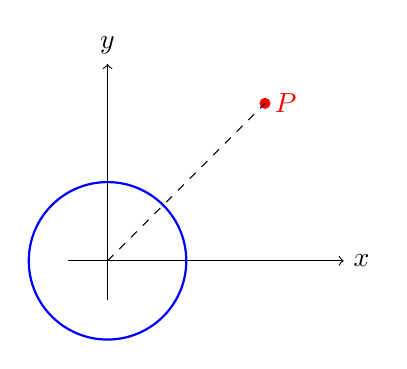
\begin{tikzpicture}
    \draw[->] (-0.5,0) -- (3,0) node[right] {$x$};
    \draw[->] (0,-0.5) -- (0,2.5) node[above] {$y$};
    \draw[thick, blue] (0,0) circle (1);
    \fill[red] (2,2) circle (2pt) node[right] {$P$};
    \draw[dashed] (0,0) -- (2,2);
  \end{tikzpicture}
  \caption{A circle, a point and a line.}
\end{figure}

\section{A pgfplots plot}

\begin{figure}[h]
  \centering
  \begin{tikzpicture}
    \begin{axis}[xlabel={$x$}, ylabel={$f(x)$}, width=8cm, legend pos=north west]
      \addplot[domain=-2:2, samples=50, blue] {x^2};
      \addplot[domain=-2:2, samples=50, red] {x^3};
      \legend{$x^2$, $x^3$}
    \end{axis}
  \end{tikzpicture}
  \caption{Two functions.}
\end{figure}

\end{document}
